% Full instructions available at:
% https://github.com/elauksap/focus-beamertheme

\documentclass[9pt]{beamer}
\usetheme{focus}

%%%%%%%%%%%%%%%%%%%%%%%%%%%%%%%%%%%%%%%%%%%%%%%%%%%%%%%%%%%%%%%%%%%%%
% Typography, change document font
\usepackage[tt=false, type1=true]{libertine}
\usepackage[varqu]{zi4}
\usepackage[libertine]{newtxmath}
\usepackage[T1]{fontenc}

\usepackage[protrusion=true,expansion=true]{microtype}

% Disable paragraph indentation, and increase gap
\usepackage{parskip}

%Matrix
\usepackage{tabstackengine}
\setstackEOL{;}% row separator
\setstackTAB{,}% column separator
\setstacktabbedgap{1ex}% inter-column gap 
\setstackgap{L}{1.0\normalbaselineskip}% inter-row baselineskip
\let\mat\bracketMatrixstack

\newcommand{\pth}{Figure/}
\newcommand{\ve}[1]{\mathbf{#1}}

% Copyright (C) 2018-2019 Pasquale Claudio Africa and the LaTeX community.
% A full list of contributors can be found at
%
%     https://github.com/elauksap/focus-beamertheme
% 
% This file is part of beamerthemefocus.
% 
% beamerthemefocus is free software: you can redistribute it and/or modify
% it under the terms of the GNU General Public License as published by
% the Free Software Foundation, either version 3 of the License, or
% (at your option) any later version.
% 
% beamerthemefocus is distributed in the hope that it will be useful,
% but WITHOUT ANY WARRANTY; without even the implied warranty of
% MERCHANTABILITY or FITNESS FOR A PARTICULAR PURPOSE. See the
% GNU General Public License for more details.
% 
% You should have received a copy of the GNU General Public License
% along with beamerthemefocus. If not, see <http://www.gnu.org/licenses/>.

\mode<presentation>


% DEFINE COLORS. ---------------------------------------------------------------
\definecolor{main}{RGB}{134, 161, 174}
\definecolor{main2}{RGB}{104, 131, 144}
\definecolor{textc}{RGB}{20, 20, 20}
\definecolor{background}{RGB}{255, 255, 255}

\definecolor{alert}{RGB}{180, 0, 0}
\definecolor{example}{RGB}{0, 110, 0}


% SET COLORS. ------------------------------------------------------------------
\setbeamercolor{normal text}{fg=textc, bg=background}
\setbeamercolor{alerted text}{fg=textc}
\setbeamercolor{example text}{fg=textc}

\setbeamercolor{titlelike}{fg=background, bg=main}
\setbeamercolor{frametitle}{parent={titlelike}}

\setbeamercolor{footline}{fg=background, bg=main2}

\setbeamercolor{block title}{bg=main!80!background, fg=background}
\setbeamercolor{block body}{bg=main!10!background, fg=textc}

\setbeamercolor{block title alerted}{bg=alert, fg=background}
\setbeamercolor{block body alerted}{bg=alert!10!background, fg=textc}

\setbeamercolor{block title example}{bg=example, fg=background}
\setbeamercolor{block body example}{bg=example!10!background, fg=textc}

\setbeamercolor{itemize item}{fg=textc}
\setbeamercolor{itemize subitem}{fg=textc}

\setbeamercolor{enumerate item}{fg=textc!70!black}
\setbeamercolor{enumerate subitem}{fg=textc!70!black}

\setbeamercolor{description item}{fg=textc!70!black}
\setbeamercolor{description subitem}{fg=textc!70!black}

\setbeamercolor{caption name}{fg=textc}

\setbeamercolor{section in toc}{fg=textc}
\setbeamercolor{subsection in toc}{fg=textc}
\setbeamercolor{section number projected}{bg=textc}
\setbeamercolor{subsection number projected}{bg=textc}

\setbeamercolor{bibliography item}{fg=main}
\setbeamercolor{bibliography entry author}{fg=main!70!black}
\setbeamercolor{bibliography entry title}{fg=main}
\setbeamercolor{bibliography entry location}{fg=main}
\setbeamercolor{bibliography entry note}{fg=main}

\mode<all>


\begin{document}
	\section{Discretisation}

	\begin{frame}
		\begin{itemize}
			\item Using either configuration, the resulting linearised quantity will be the same
			\item Spatial is easier though
			
		\end{itemize}
	\end{frame}


	\begin{frame}{Discretised kinematics}
		\begin{itemize}
			\item Isoparametric elemnents, discretise the initial geometry $X$, defomrned geometry $x$, virtual velocity $v, \delta v$ and linearised displacment $u$
			
			\begin{equation}
				\begin{aligned}
				X = N_aX_a\\
				x = N_ax_a\\
				v =  N_av_a\\
				\delta v = N_a \delta v_a\\
				u = N_a u_a
				\end{aligned}
			\end{equation}
			where a = 1...n Number of nodes in element, and $N(\xi_1,\xi_2,\xi_3)$ are the standard shape parametric shape function
		\end{itemize}
	\end{frame}

	\begin{frame}
		\begin{itemize}
			\item  The deformation gradiend F is interpolated over an element
			\begin{equation}
			\ve{F = \sum_{i}^{n}x_a \otimes \nabla_o N_a}
			\end{equation}
			$F = \mat{\frac{\partial x_1}{\partial X_1},\frac{\partial x_1}{\partial X_2},\frac{\partial x_1}{\partial X_3} ; , , ;
					  \frac{\partial x_2}{\partial X_1},\frac{\partial x_2}{\partial X_2},\frac{\partial x_2}{\partial X_3}; , , ;
				  	  \frac{\partial x_3}{\partial X_1},\frac{\partial x_3}{\partial X_2},\frac{\partial x_3}{\partial X_3}}$
			\qquad $\ve{x = N_ax_a}$ , so $\ve{\mat{x_1;x_2;x_3} = N_a\mat{x_{a_1};x_{a_2} ;x_{a_3} }}$ 			\\ and $\frac{\partial x_1}{\partial X_1} =  \frac{\partial N_a x_{a_1}}{\partial X_1}$
			\item $F_{iJ} = \sum_{a}^{n} x_{a,i} \frac{\partial N_a}{\partial X_J} \quad$ $i$ is the component of the deflection given as descritised, and j is the component of the deformed geometry. AGAIN descritised! 
			\item where $\nabla_o N_a = \frac{\partial N_a}{\partial \ve{X}}$ 
			\item We can relate it to $\nabla_{\xi} N_a = \frac{\partial N_a}{\partial \ve{\xi}}$ using chain rule as\\
			$\frac{\partial N_a}{\partial \ve{X}} = \left(\frac{\partial X}{\partial \ve{\xi}} \right)^{-T}\frac{\partial N_a}{\partial \ve{\xi}}$ \qquad ($\frac{\partial N}{\partial \xi} = \frac{\partial N}{\partial \ve{X}}\frac{\partial \ve{X}}{\partial \xi}$) \qquad ($\frac{\partial N_1}{\partial \xi_1} = \frac{\partial N_1}{\partial X_1}\frac{\partial X_1}{\partial \xi_1} + \frac{\partial N_1}{\partial X_3}\frac{\partial X_3}{\partial \xi_1}+ \frac{\partial N_1}{\partial X_2}\frac{\partial X_2}{\partial \xi_1}$) \\ 
			$\frac{\partial \ve{X}}{\partial \ve{\xi}} =  \sum_{i}^{n}X_a \otimes \nabla_{\xi} N_a$ 
			\qquad  \qquad 
			$\ve{\frac{\partial X}{\partial \xi} = \mat{\frac{\partial X_1}{\partial \xi_1},\frac{\partial X_1}{\partial \xi_2},\frac{\partial X_1}{\partial \xi_3} ; , , ;
			\frac{\partial X_2}{\partial \xi_1},\frac{\partial X_2}{\partial \xi_2},\frac{\partial X_2}{\partial \xi_3}; , , ;
			\frac{\partial X_3}{\partial \xi_1},\frac{\partial X_3}{\partial \xi_2},\frac{\partial X_3}{\partial \xi_3}}}$

		\end{itemize}	\end{frame}
	
	
	\begin{frame}{Defomration mesaures}
		\begin{itemize}
			\item We can work also with the right and left Cauchy tensors $\ve{C}$ and $\ve{b}$
			\begin{equation}
			\begin{aligned}
			\ve{C =  F^TF = \sum_{a,b}^{} (x_a.x_b) \nabla_o N_a \otimes \nabla_o N_b}\\
			\ve{b =  FF^T = \sum_{a,b}^{} (\nabla_o N_a.\nabla_o N_b)  x_a \otimes x_b}
			\end{aligned}
			\end{equation}
			\item We also know that the velocity gradient $\ve{d = \frac{1}{2}\left(l+l^T \right)}$ can be given as
			\begin{equation}
			\begin{aligned}
			\ve{d = \frac{1}{2}\left( v_a \otimes \nabla N_a + \nabla N_a \otimes v_a \right)}\\
			\ve{\delta d = \frac{1}{2}\left( \delta v_a \otimes \nabla N_a + \nabla N_a \otimes \delta v_a \right)} \footnote{Variation is in the DOF not in N}\\
			\varepsilon =  \frac{1}{2}\left( u_a \otimes \nabla N_a + \nabla N_a \otimes u_a \right)
			\end{aligned}
			\end{equation}
			So basically whenever we are finding the derivative of the continuous funciton, we replace it with the discretise one! Representing the derivative of N in parametric form, as:
			\begin{equation}
			\begin{aligned}
			\frac{\partial N_a}{\partial \ve{x}} = \left( \frac{\partial \ve{x}}{\partial \xi}\right)^{-T} ; \frac{\partial N_a}{\partial \xi} = \sum_{a}^{n} x_a \otimes \nabla_\xi N_a; \frac{\partial x_i}{\partial \xi_\alpha} = \sum_{a}^{n} x_{a,i} \frac{\partial N_a}{\partial \xi_\alpha}
			\end{aligned}
			\end{equation}	
		\end{itemize}
	\end{frame}


	\begin{frame}{Problem \#1}
		\begin{figure}
			\centering
			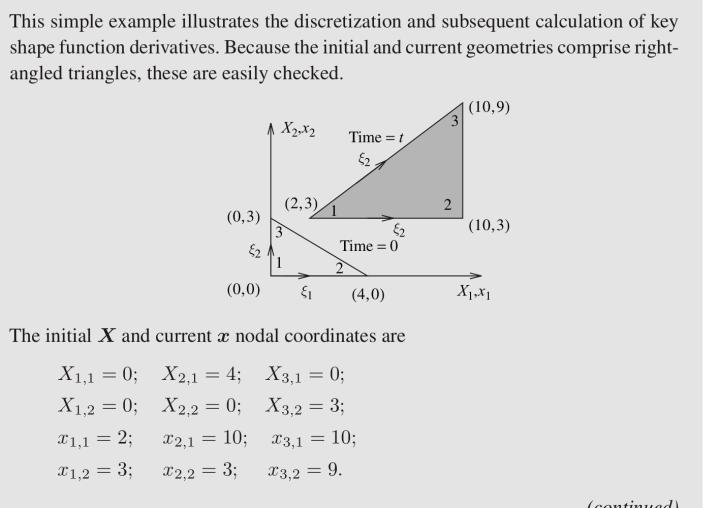
\includegraphics[width=0.5\linewidth]{Figure/fig12}
		\end{figure}
		\begin{itemize}
			\item The shape function are 
			\begin{equation}
				\begin{aligned}
				N_1 = 1 - \xi_1 + \xi_2;\qquad N_2 = \xi_2;\qquad N_3 = \xi_2 \\
				\frac{\partial N_1}{\partial \xi} = \mat{-1;-1} \qquad \frac{\partial N_2}{\partial \xi} = \mat{1;0} \qquad \frac{\partial N_3}{\partial \xi} = \mat{0;1} 
				\end{aligned}
			\end{equation}
			Also
			\begin{equation}
			X = N_a(\xi) X_a \qquad X_1 = 4\xi_1 \qquad X_2 = 3\xi_2
			\end{equation}
			Think of $N(\xi)$ like some scaling that takes X to the actual value $X_a$. Like a mapper (maybe lienar or not) from 0 to 1 that makes you actually move in the X space.
		\end{itemize}
	\end{frame}

	\begin{frame}
		\begin{itemize}
			\item $\frac{\partial \ve{X}}{\partial \xi} = \mat{4,0;0,3}\qquad  \left(\frac{\partial \ve{X}}{\partial \xi} \right)^{-T} = \frac{1}{12}\mat{3,0;0,4}$ 
			\item $\frac{\partial N_a}{\partial \ve{X}} = \left(\frac{\partial X}{\partial \ve{\xi}} \right)^{-T}\frac{\partial N_a}{\partial \ve{\xi}}$
			
			\begin{equation}
				\begin{aligned}
				\frac{\partial N_1}{\partial \ve{X}} = \frac{1}{12}\mat{3,0;0,4}\mat{-1;-1} = \frac{-1}{12}\mat{3;4} \qquad 	\frac{\partial N_2}{\partial \ve{X}}  = \frac{1}{12}\mat{3;0} \qquad \frac{\partial N_3}{\partial \ve{X}}  = \frac{1}{12}\mat{0;4}
				\end{aligned}
			\end{equation}
			 \item We can do the same with respect to the spatial coordinates giving us
			 			\begin{equation}
			 \begin{aligned}
			 \frac{\partial N_1}{\partial \ve{x}} = \frac{1}{24}\mat{3,0;-4,4}\mat{-1;-1} = \frac{-1}{24}\mat{3;0} \qquad 	\frac{\partial N_2}{\partial \ve{x}}  = \frac{1}{24}\mat{3;-4} \qquad \frac{\partial N_3}{\partial \ve{x}}  = \frac{1}{24}\mat{0;4}
			 \end{aligned}
			 \end{equation}
			 \item $F_{iJ} = \sum_{a}^{n} x_{a,i} \frac{\partial N_a}{\partial X_J} $
			 \item $F_{11} = x_{1,1}\frac{\partial N_1}{\partial X1} + x_{2,1}\frac{\partial N_2}{\partial X1} + x_{3,1}\frac{\partial N_3}{\partial X1} = \frac{1}{12}\left(-2.3 +10.3+10.0\right) =\frac{6}{3}$
			 \item $\ve{F} = \frac{1}{3}\mat{6,8;0,6}$
			 \item $\ve{C = F^TF \qquad b = FF^T \qquad \text{J = det}F}$
		\end{itemize}
	\end{frame}

	\begin{frame}{Discretised equilibrium}
		\begin{block}{Spatial description}
			\begin{equation}
				\delta W(\phi,\delta v) = \int_v \sigma : \delta d dv - \int_v f. \delta v dv - \int_{\Gamma} t. \delta v da
			\end{equation}
			which is the virtual work done by the residual $\ve{r}$. \\
			A pretty neat thing is that we can consider a single virtual nodal velocity $\delta v_a$ occuring at node $a$ in element $e$. We will assemble the elements later but the velocity at the node will be consistent.
			\begin{equation}
			\delta W^e(\phi,N_a\delta v_a) =  \int_{v^e} \ve{\sigma} : (\delta v_a \otimes \nabla N_a) dv - \int_{v^e} f. (N_a \delta v_a) dv - \int_{\Gamma^e} t. (N_a \delta v_a)da
			\end{equation}
			* Very interesting, this gives us the equilibrium at a node $a$. The $\nabla N_a$ almost acts like a component term  \\
			* The first term because $\sigma$ is symmetric so the 1/2 in velocity gradient disappears\\
		\end{block}
	
		Insight :
		\begin{equation}
			\begin{aligned}
			d = \frac{1}{2}\left(l  + l^T \right) = \frac{1}{2}\left(\nabla v + (\nabla v)^T \right) \\
			\nabla v = n_a \otimes \nabla N_a \text{CHECK????}
			\end{aligned}
		\end{equation}
	\end{frame}


	\begin{frame}
		We know that $\ve{\sigma :(u \otimes v) = u. \sigma v}$ for any vectors $\ve{v,u}$. Almost like when you take a scalar product and you only want the diagonals added
		
		So we get 
		\begin{equation}
			\delta W^e(\phi,N_a\delta v_a) =  \delta v_a .\left(\int_{v^e} \ve{\sigma} \nabla N_a dv - \int_{v^e} N_af dv - \int_{\Gamma^e} N_a tda \right)
		\end{equation}
		
		$\delta v_a = \mat{\delta v_{a,1} ; \delta v_{a,2}; \delta v_{a,3}}$\\
		
		\begin{itemize}
			\item So per element the virtual work is expressed in terms of the internal and external nodal forces $\ve{T_a^e}$ and $\ve{F_a^e}$
			\item $ \delta W^e(\phi,N_a\delta v_a) = \ve{\delta v.(T_a^e-F_a^e)}$ \\
			$\ve{T_a^e} ~\text{is the internal force with different components }, T_{a,i}^e = \sum_{j}^{3} \int_{v^e} \sigma_{ij}\frac{\partial N_a}{\partial x_j} dv$ ($\sigma \nabla N_a$ is a linear map where $\nabla N_a$ is a vector, but with respect to the global directions!. But it's not a unit vector)	
			\item The cauchy stress is found from the constitutive relationship and the left cauchy tensor	
			\item The virtual work allows you to say that the components of the inernal forces will be zero
		\end{itemize}
	\end{frame}


	\begin{frame}{Problem \#2}
		\begin{itemize}
			\item Same example as last where $b = \frac{1}{9} \mat{100,48,0;48,36,0;0,0,9}$ and J = 4
			\item $\sigma =  \mat{\sigma_{11},\sigma_{12},0;\sigma_{21},\sigma_{22},0;
			0,0,\sigma_{33}} = \frac{\mu}{J}(b-I) + \frac{\lambda}{J}(lnJ)I = \mat{8,4,0;4,3,0;0,0,0.8}$
			\item $T_{a,i} = \int_{v^e} \left(\sigma_{i1} \frac{\partial N_a}{\partial x_1} + \sigma_{i2} \frac{\partial N_a}{\partial x_2} \right)$ dv \\
			\item $ T_{1,1} = -24t \qquad T_{1,1} = 8t \qquad T_{1,1} = 16t $ \\ 
				  $	T_{1,2} = -12t \qquad T_{2,2} = 0 \qquad T_{3,2} = 12t $	 		
		\end{itemize}
 	\end{frame}
 
 
 	\begin{frame}
 		Equilibrium at a global level :
 		\begin{itemize}
 			\item From all elements e (1 to $m_1$) containing node $a$ \\
 			$\delta W(\phi,N_a \delta v) = \sum_{e=1,e \ni a}^{m_a} \delta W^e(\phi,N_a \delta \ve{v_a}) = \delta \ve{v_a . (T_a-F_a)}$ 	
 			\item where assembled equivalent nodal forces are:		
 			$\ve{T_a =\sum_{e=1,e \ni a}^{m} T_a^e \qquad F_a =\sum_{e=1,e \ni a}^{m} F_a^e  }$
 			\item And then for all nodes we get
 			$\delta W(\phi,\delta v) = \sum_{a}^{n} \ve{\delta v_a . \left(T_a -F_a \right)}$
 			\item Since the virtual work should be satisifed for any virtual nodal velocity, we get the Residual force with respect to the whole system
 			$\ve{R_a = T_a - F_a}$
 		\end{itemize}
 	\end{frame}
 
 	\begin{frame}{Matrix notation}
 		\begin{itemize}
 			\item Organise $R$ in an array $\ve{T=[T_1~T_2...T_N],F = [...] ,R = [....]}$ (I think each $T_1$ contains three components)
 			\item Virtual work equation is : $ \ve{\delta v^TR = \delta v^T(T-F) = 0}$\\
 			where $\ve{\delta v^T = [\delta v_1^T \delta v_2^T....]}$
 			\item Since the internal forces are nonlinear functions of the current nodal positions $\ve{x = [x_1 x_2 x_3 ...]}$
 			\item In matrix notation, we keep the symmetric tensor as $\sigma' = [ \sigma_{11},\sigma_{22},\sigma_{33},\sigma_{12},\sigma_{13},\sigma_{23}]^T$ and $\ve{d}$ as $\ve{d} = [ d_{11},d_{22},d_{33},2d_{12},2d_{13},2d_{23}]^T$ (Where off diagonals is twice to make sure $d^T \sigma$ gives the correct internal energy)
 			\item $\ve{\int \sigma:d = \int d^T\sigma }dv$
 			\item $\ve{d = \sum_{a}^{n}B_av_a}$ where $B_a = \mat{\frac{\partial N_a}{\partial x_1},0,0; 0,\frac{\partial N_a}{\partial x_2},0;0,0,\frac{\partial N_a}{\partial x_3};
 				\frac{\partial N_a}{\partial x_2},\frac{\partial N_a}{\partial x_1},0; , , ;
 				\frac{\partial N_a}{\partial x_3},0,\frac{\partial N_a}{\partial x_1};
 				0,\frac{\partial N_a}{\partial x_3},\frac{\partial N_a}{\partial x_2}}$

 		\end{itemize}
 	\end{frame}
 
 	\begin{frame}
 		\begin{itemize}
 			\item So : $\delta W = \int (B_a \delta v_a)^T \sigma dv - \int f.(N_a \delta v_a) dv - \int t.(N_a \delta v_a) da$ 
 			\item We can also write the internal force as : $T_a^e = \int_{v^e} B^T_a \sigma' dv$
 			
 		\end{itemize} 
 	\end{frame}
 
 
 	\begin{frame}{Discretisation of linearised equilibrium equations}
 		\begin{itemize}
 			\item The equilibrium equations are still nonlinear with respect to the nodal positions. A NR is used to solve it
 			\item The linear virtual work components is found using the directional derivative as 
 			\begin{equation}
 			D\delta W(\phi,\delta v)[u] = D \delta W_{int}(\phi,\delta v)[u] - D \delta W_{ext}(\phi,\delta v)[u]
 			\end{equation}
 			\item The internal work linearisation can be decomposed into the constitutive and intial stress components
 			\begin{equation}
 			D \delta W_{int}(\phi,\delta v)[u] =D \delta W_{C}(\phi,\delta v)[u] +D \delta W_{\sigma}(\phi,\delta v)[u] 
 			\end{equation}
 			\begin{equation}
 			 = \ve{\int_v \delta d:c:\varepsilon} dv + \ve{\int_v \sigma : \left((\nabla u)^T(\nabla \delta v) \right)} dv
 			\end{equation}
 			which is the tangent stiffness matrix
 			\end{itemize}
 	\end{frame}
 
 
 	\begin{frame}
 		\begin{itemize}
 			\item Remember that at each node, we get the residual due to the nodal equivalent forces at $a$ due to the whole equilibrium of node $a$ (R = T -F)
 			\item F may be dependant on $a$ and so linearisation in the direction of $u_b$ or $N_bu_b$ with $N_av_a$ constant, gives only the change of the residual force at node a due to the change $u_b$ in the current position of node $b$
 			\begin{equation}
 			D\delta W^e(\phi,N_a\delta v_a)[N_bu_b] = D(\delta v_a.(T_a^e - F_a^e))[N_bu_b]
 			\end{equation}
 			\begin{equation}
 			 = \delta v_a.D(T_a^e - F_a^e)[N_bu_b] = \delta v_a.K^e_{ab}u_b
 			\end{equation}
 			\item Change in force at node $a$ due to change in current position of node $b$
 			\item This is not the full stiffness matrix, but each component. When we do the whole assembly, we get the full tangen stiffness matrix
 			
 			\begin{equation}
 				\frac{\partial \ve{R}}{\partial \ve{U}} = \mat{\frac{\partial R_1}{\partial u_1},\frac{\partial R_1}{\partial u_2},.....,\frac{\partial R_1}{\partial u_n};
 					 , , , ;
 				\frac{\partial R_2}{\partial u_1},\frac{\partial R_2}{\partial u_2},.....,\frac{\partial R_2}{\partial u_n};
 				 , , , ;
	 			\frac{\partial R_n}{\partial u_1},\frac{\partial R_n}{\partial u_2},.....,\frac{\partial R_n}{\partial u_n}}
 			\end{equation}
 			So one component here is attained by finding the linearisation in one direction node with the virtual work equilibrium in another node seperately
 		\end{itemize}
 	\end{frame}
 
 
 	\begin{frame}{Consititutive component:Indices}
 		\begin{itemize}
 			\item Check bonet page 248
 			\item 
 			\begin{equation}
 			D\delta W_c^e(\phi,N_a\delta v_a)[N_bu_b] = \delta va. K^e_{c,ab} u_b
 			\end{equation}
 			\item where
 			\begin{equation}
 			[K_{c,ab}]_{ij} = \int_{v^e} \sum_{k,l=1}^{3} \frac{\partial N_a}{\partial x_k} Cikjl \frac{\partial N_b}{\partial x_l} dv \qquad i,j = 1,2,3
 			\end{equation}
 		\end{itemize}
 	\end{frame}
 
 
 	\begin{frame}{Problem \#3 : Find tangent stifness components between node 2 and 3}
		\begin{figure}
 			\centering
 			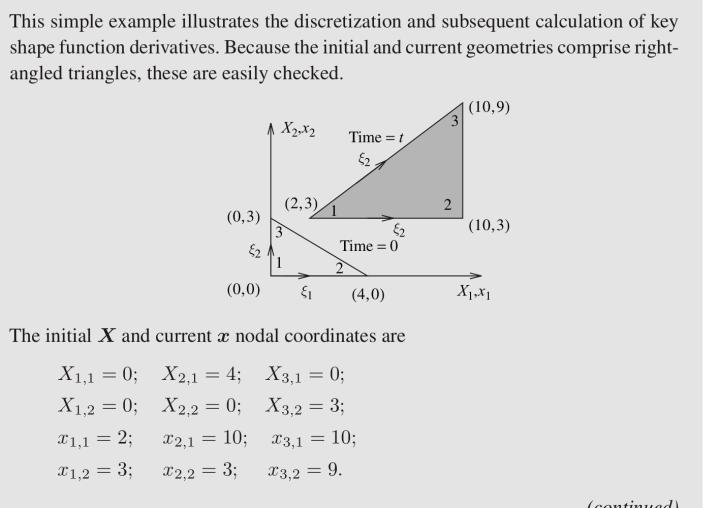
\includegraphics[width=0.45\linewidth]{Figure/fig12} 	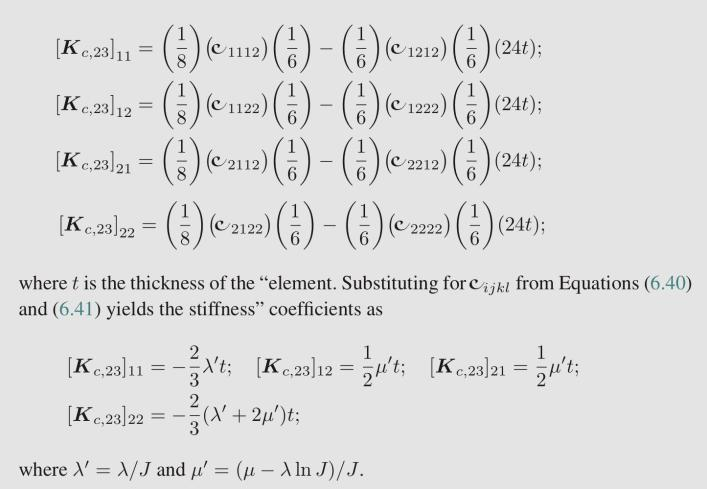
\includegraphics[width=0.5\linewidth]{Figure/fig13}
 		\end{figure}
 	
 		{\tiny
		\begin{equation}
		 	\begin{aligned}
		 	\frac{\partial N_1}{\partial \ve{x}} = \frac{1}{24}\mat{3,0;-4,4}\mat{-1;-1} = \frac{-1}{24}\mat{3;0} \qquad 	\frac{\partial N_2}{\partial \ve{x}}  = \frac{1}{24}\mat{3;-4} \qquad \frac{\partial N_3}{\partial \ve{x}}  = \frac{1}{24}\mat{0;4}
	 	\end{aligned}
 		\end{equation}}
 	
 	$K_{11}$ means equilibrium in 2 due to change in 3
 	\end{frame}
 
 
 	\begin{frame}{Constitutive component:Matrix form}
 		\begin{itemize}
 			\item Virtual work for element $e$ expressed in matrix notation by a small starin vector as 
 			$\varepsilon' = [\varepsilon_{11},\varepsilon_{22},\varepsilon_{33},2\varepsilon_{12},2\varepsilon_{13},2\varepsilon_{23}]^T$
 			\item $\varepsilon' = B_au_a$
 			\item Now the constitutive component of the linearised virtual work can be written as
 			\begin{equation}
 			D\delta W_C(\phi,\delta v)[u] = \int_V \delta d :c:\varepsilon dv = \int_v \delta \ve{d^TD\varepsilon}' dv
 			\end{equation}
 			\item Where the later part is the matrix componets received from the tensor contraction
 			\begin{equation}
 				D = \mat{c_{1111},c_{1122},c_{1133},c_{1112},c_{1113},c_{1123};
 						 c_{2211},c_{2222},c_{2233},c_{2212},c_{2213},c_{2223};
 						 .,.,.,.,.,.;
 					     c_{2311},c_{2322},c_{2333},c_{2312},c_{2313},c_{2323}}
 			\end{equation}
 			\item See bonet page 250 for neo-Hookean model
 			\item For node a and b
 			\begin{equation}
 				D\delta W_c^e(\phi,N_a\delta v_a)[N_b u_b] = \int_{v^e} \ve{(B_a \delta v_a)^TD(B_b u_b)} dv =  \underset{Tangent~ K}{\int_{v^e} \ve{\delta v_a.(B_a ^TDB_b ).u_b} dv}
 			\end{equation}
 		\end{itemize}
 	\end{frame}
 
 
 	\begin{frame}{Initial stress component}
 		\begin{itemize}
 			\item Remember that the gradients of $u$ and $\delta v$ can be found as
 			\begin{equation}
 				\begin{aligned}
 				\nabla \delta \ve{v} = \delta v_a \otimes \nabla N_a \\
 				\nabla \delta \ve{u} = \delta u_b \otimes \nabla N_b \\
 				\end{aligned}
 			\end{equation}
 			\item We've seen the intial stress component as (Check the linearising equilib equations)
 			\begin{equation}
 			\begin{aligned}
	 			D \delta W_{\sigma}(\phi,N_a\delta v_a)[N_b \delta u_b] = \int_v \ve{\sigma:[(\nabla u_b)^T \nabla \delta v_a] dv} \\
	 			= \int_v \ve{\sigma:[(\delta v_a . u_b)} \nabla N_b \otimes \nabla N_a] dv \\
	 			= (\delta v_a. u_b) \int_{v^e} \nabla N_a .\sigma \nabla N_b dv
	 			 			\end{aligned}
 			\end{equation}
 			\item  As we have $\delta v_a.u_b = \delta v_a.Iu_b$
 			\item  We get $\delta v_a . K_{\sigma, ab} u_b$
 			\begin{equation}
 				\begin{aligned}
 				\ve{K^e_{\sigma,ab} = \int_{v^e} (\nabla N_a.\sigma \nabla N_b)I dv}\\
 				[K^e_{\sigma,ab}]_{ij} = \int_{v^e} \sum_{k,l=1}^{3} (\frac{\partial N_a}{\partial x_k} \sigma_{kl} \frac{\partial N_b}{\partial x_l}\delta_{ij}) dv
 				\end{aligned}
 			\end{equation}
 		\end{itemize}
 	\end{frame}
 
 
 	\begin{frame}{Problem \#3}
 		\begin{itemize}
 			\item Find intial stiffness matrix joining node 1 and 2 
 			\begin{equation}
 			[K_{\sigma,12}] = \int_{v^e} \mat{\frac{\partial N_1}{\partial x_1},\frac{\partial N_1}{\partial x_2}} \mat{\sigma_{11},\sigma_{12};\sigma_{21},\sigma_{22}}
 			\mat{\frac{\partial N_2}{\partial x_1};\frac{\partial N_2}{\partial x_2}}
 			\mat{1,0;0,1} dv
 			\end{equation}
 			
 		\end{itemize}
 	\end{frame}
 
 
 	\begin{frame}{External force}
 		Check bonet : 252
 	\end{frame}
 
 
 	\begin{frame}{Tangent matrix}
		\begin{figure}
 			\centering
 			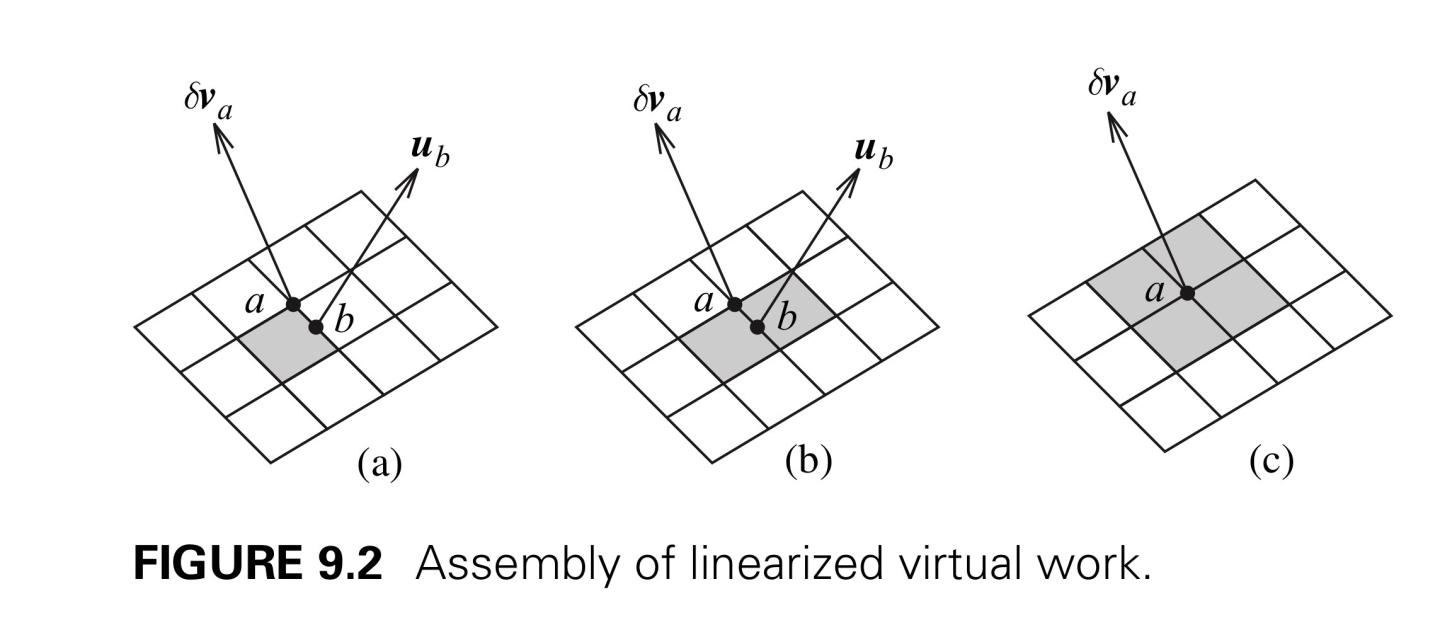
\includegraphics[width=0.5\linewidth]{Figure/fig14} 
 		\end{figure}
	 	\begin{itemize}
			\item For an element $e$ linking nodes a and b we find $\ve{K_{ab}^e = K_{c,ab}^e + K_{\sigma,ab}^e + K_{p,ab}^e}$  (Fig a)
	 		\item Then we find the assembly of the total linearized virtual work of contribution to a from b from all elements (Fig b)
	 		\item Find then for all nodes connecting to a
	 		\item Doing the above for all nodes
	 	\end{itemize}
 	
 	\begin{equation}
 	\tiny
 		\begin{aligned}
 		(i) D\delta W(\phi,N_a\delta v_a)[N_bu_b] = \sum_{e=1,e \ni a,b}^{m_{a,b}} D\delta W^e(\phi,N_a \delta v_a)[N_b u_b]\\
 		(ii)  D\delta W(\phi,N_a\delta v_a)[u] = \sum_{b=1}^{n_a} D\delta W^e(\phi,N_a \delta v_a)[N_b u_b]\\
 		(iii)  D\delta W(\phi,v)[u] = \sum_{a=1}^{N} D\delta W^e(\phi,N_a \delta v_a)[u]\\
 		\end{aligned}
 	\end{equation}
 	$n_a$ is no of nodes connected to $a$
 	\end{frame}
 
 	
 	\begin{frame}{Solvers}
 		Check bonet 258 for 
 		\begin{itemize}
 			\item NR
 			\item Line search
 			\item Arc-Length method 			
 		\end{itemize}
 	\end{frame}
 
\end{document}